\section{K : Pointers}
\label{chap:pointers}

%%%%%%%%%%%%%%%%%%%%%%%%%%%%%%%%%%%%%%%%%%%%%%%%%%%%%%%%%%%%%%

\begin{frame}[fragile]
\frametitle{Call-by-Value}
\begin{columns}[T]

\begin{column}{0.45\textwidth}
\lstinputlisting[style=basicc]{../Code/ChapK/callbyval.c}
\outputlisting{../Code/ChapK/callbyval.autoout}
\end{column}

\pause
\begin{column}{0.45\textwidth}
\begin{itemize}[<+->]
\item In the program, the function cannot change
the value of \verb^v^ as defined in \verb^main()^ since
a {\bf copy} is made of it.
\item To allow a function to modify the value of a variable
passed to it we need a mechanism known as
{\bf call-by-reference}, which uses the {\bf address}
of variables (pointers). 
\end{itemize}
\end{column}

\end{columns}
\end{frame}


%%%%%%%%%%%%%%%%%%%%%%%%%%%%%%%%%%%%%%%%%%%%%%%%%%%%%%%%%%%%%%

\begin{frame}[fragile]
\frametitle{Call-by-Reference}
\begin{columns}[T]

\begin{column}{0.45\textwidth}
\begin{itemize}[<+->]
\item We have already seen addresses used with \verb^scanf()^.
The function call:
\begin{verbatim}
scanf("%i", &v);
\end{verbatim}
causes the appropriate value to be stored at a particular
address in memory.
\item If \verb^v^ is  a variable, then \verb^&v^ is its
address, or location, in memory.
\end{itemize}
\end{column}

\pause
\begin{column}{0.45\textwidth}
\begin{itemize}[<+->]
\item
\begin{verbatim}
int i, *p;
\end{verbatim}
\item Here \verb^i^ is an \verb^int^ and \verb^p^ is of type
{\it pointer to int}.
\item Pointers have a legal range which
includes the special address \verb^0^ and a set of positive
integers which are the machine addresses of a particular
system.
\end{itemize}
\begin{center}
\begin{figure}[h]
\centerline{
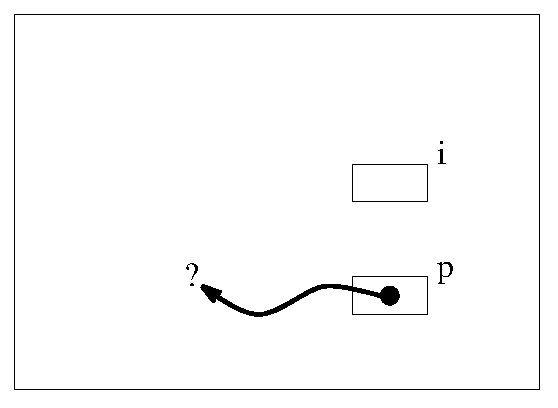
\includegraphics[scale=0.40]{../Figs/point8_1.eps}
}
\end{figure}
\end{center}
\end{column}

\end{columns}
\end{frame}

%%%%%%%%%%%%%%%%%%%%%%%%%%%%%%%%%%%%%%%%%%%%%%%%%%%%%%%%%%%%%%

\begin{frame}[fragile]
\frametitle{The {\em NULL} Pointer}
\begin{columns}[T]

\begin{column}{0.45\textwidth}
\begin{itemize}[<+->]
\item 
\begin{verbatim}
p = NULL;
\end{verbatim}
\end{itemize}
\begin{center}
\begin{figure}[h]
\centerline{
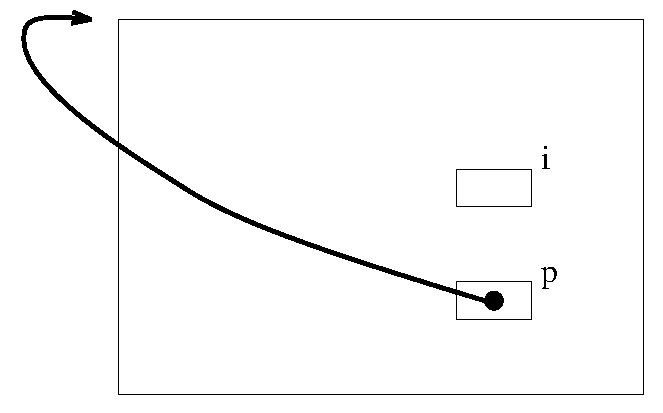
\includegraphics[scale=0.40]{../Figs/point8_2.eps}
}
\end{figure}
\end{center}
\end{column}

\pause
\begin{column}{0.45\textwidth}
\begin{itemize}[<+->]
\item 
\begin{verbatim}
p = &i;
\end{verbatim}
\end{itemize}
\begin{center}
\begin{figure}[h]
\centerline{
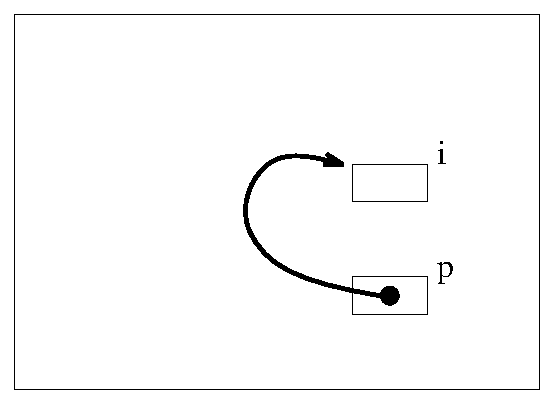
\includegraphics[scale=0.40]{../Figs/point8_3.eps}
}
\end{figure}
\end{center}
\end{column}

\end{columns}
\end{frame}

%%%%%%%%%%%%%%%%%%%%%%%%%%%%%%%%%%%%%%%%%%%%%%%%%%%%%%%%%%%%%%

\begin{frame}[fragile]
\frametitle{Equivalence of {\em i} and {\em *p}}
\begin{columns}[T]

\begin{column}{0.45\textwidth}
\begin{itemize}[<+->]
\item 
\begin{verbatim}
i = 5;
\end{verbatim}
\end{itemize}
\begin{center}
\begin{figure}[h]
\centerline{
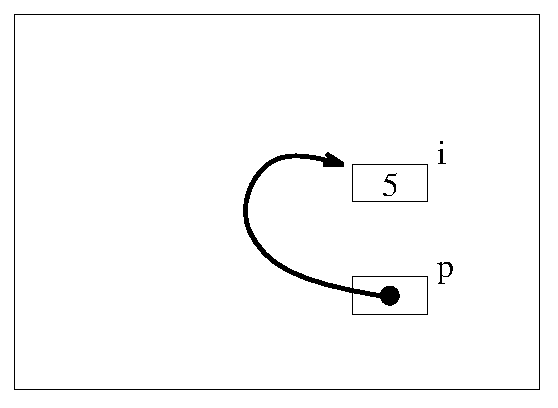
\includegraphics[scale=0.40]{../Figs/point8_4.eps}
}
\end{figure}
\end{center}
\end{column}

\pause
\begin{column}{0.45\textwidth}
\lstinputlisting[style=basicc]{../Code/ChapK/pointer1.c}
\outputlisting{../Code/ChapK/pointer1.autoout}
\end{column}

\end{columns}
\end{frame}

%%%%%%%%%%%%%%%%%%%%%%%%%%%%%%%%%%%%%%%%%%%%%%%%%%%%%%%%%%%%%%

\begin{frame}[fragile]
\frametitle{{\em scanf} Again}
\begin{columns}[T]

\begin{column}{0.45\textwidth}
\lstinputlisting[style=basicc]{../Code/ChapK/pointer2.c}
\outputlisting{../Code/ChapK/pointer2.manout}
\end{column}

\pause
\begin{column}{0.45\textwidth}
\begin{itemize}[<+->]
\item In many ways the dereference operator \verb^*^ is
the inverse of the address operator \verb^&^.
\lstinputlisting[style=basicc,linerange={6-8},numbers=none]{../Code/ChapK/pointer3.c}
\item What is this equivalent to~?
\end{itemize}
\end{column}

\end{columns}
\end{frame}

%%%%%%%%%%%%%%%%%%%%%%%%%%%%%%%%%%%%%%%%%%%%%%%%%%%%%%%%%%%%%%

\begin{frame}[fragile]
\frametitle{The {\em swap} Function}
\begin{columns}[T]

\begin{column}{0.45\textwidth}
\lstinputlisting[style=basicc]{../Code/ChapK/swap.c}
\outputlisting{../Code/ChapK/swap.autoout}
\end{column}


\pause
\begin{column}{0.45\textwidth}
\begin{itemize}[<+->]
\item At beginning of function:
\begin{center}
\begin{figure}[h]
\centerline{
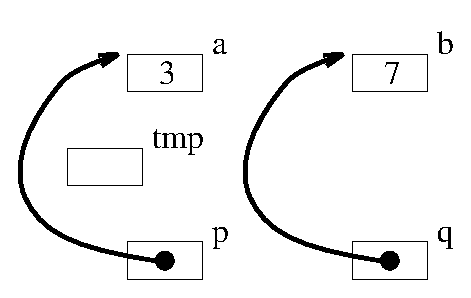
\includegraphics[scale=0.40]{../Figs/point8_7.eps}
}
\end{figure}
\end{center}

\item At end of function:
\begin{center}
\begin{figure}[h]
\centerline{
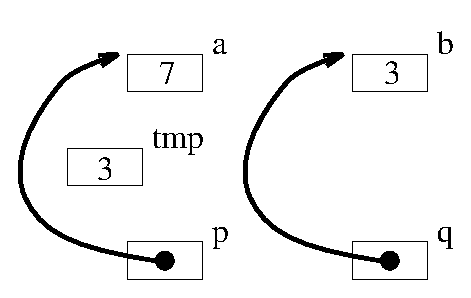
\includegraphics[scale=0.40]{../Figs/point8_8.eps}
}
\end{figure}
\end{center}
\item Remember that the variables $a$ and $b$ are not in the scope of
{\em swap()}.
\end{itemize}

\end{column}

\end{columns}
\end{frame}


%%%%%%%%%%%%%%%%%%%%%%%%%%%%%%%%%%%%%%%%%%%%%%%%%%%%%%%%%%%%%%


\begin{frame}[fragile]
\frametitle{Arrays are Pointers~?}
\begin{columns}[T]

\begin{column}{0.45\textwidth}
\begin{itemize}[<+->]
\item An array name by itself is simply an address
({\bf Array Decay}).

\item 
For instance:
\begin{verbatim}
int a[5];
int *p;
\end{verbatim}
declares an array of \verb^5^ elements, and
\verb^a^ is the address of the start of the
array.
\item
Assigning:
\begin{verbatim}
p = a;
\end{verbatim}
is completely valid and
the same as:
\begin{verbatim}
p = &a[0];
\end{verbatim}
\end{itemize}
\begin{center}
\begin{figure}[ht]
\centerline{
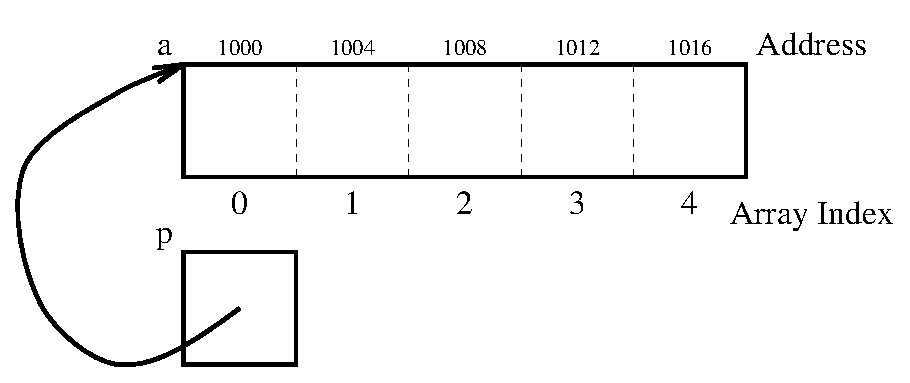
\includegraphics[scale=0.25]{../Figs/array9_2.eps}
}
\end{figure}
\end{center}
\end{column}


\pause
\begin{column}{0.45\textwidth}
\begin{itemize}[<+->]
\item To assign \verb^p^ to point to the next element,
we could either~:
\begin{verbatim}
p = a + 1;
p = &a[1];
\end{verbatim}
\item Notice that \verb^p = a + 1^ advances
the pointer {\bf 4} bytes and not 1 byte.
This is because an integer is 4 bytes long and
\verb^p^ is a pointer to an int.
\item we can use the pointer \verb^p^ is exactly
the same way as normal, i.e.:
\begin{verbatim}
*p = 5;
\end{verbatim}
\end{itemize}
\end{column}

\end{columns}
\end{frame}

%%%%%%%%%%%%%%%%%%%%%%%%%%%%%%%%%%%%%%%%%%%%%%%%%%%%%%%%%%%%%%

\begin{frame}[fragile]
\frametitle{Summing an Array}
\begin{columns}[T]

\begin{column}{0.30\textwidth}
\lstinputlisting[style=basicc]{../Code/ChapK/sum1.c}
\outputlisting{../Code/ChapK/sum1.autoout}
\end{column}

\pause
\begin{column}{0.30\textwidth}
\lstinputlisting[style=basicc]{../Code/ChapK/sum2.c}
\outputlisting{../Code/ChapK/sum2.autoout}
\end{column}

\pause
\begin{column}{0.30\textwidth}
\lstinputlisting[style=basicc]{../Code/ChapK/sum3.c}
\outputlisting{../Code/ChapK/sum3.autoout}
\end{column}

\end{columns}
\end{frame}

%%%%%%%%%%%%%%%%%%%%%%%%%%%%%%%%%%%%%%%%%%%%%%%%%%%%%%%%%%%%%%

\begin{frame}[fragile]
\frametitle{Pointers to Structures}
\begin{columns}[T]

\begin{column}{0.30\textwidth}
\begin{itemize}[<+->]
\item By default, structures are passed by value (copied) when used as a parameter to a function.
\item But, like any other type, we could pass a pointer instead.
\item The complication is that to access the elements of a structure via a pointer, we use the ``\verb^->^'' operator, and not the ``\verb^.^''.
\end{itemize}
\end{column}

\pause
\begin{column}{0.60\textwidth}
\lstinputlisting[style=basicc,linerange={58-78},numbers=none]{../Code/ChapK/cards5.c}
\end{column}

\end{columns}
\end{frame}


%%%%%%%%%%%%%%%%%%%%%%%%%%%%%%%%%%%%%%%%%%%%%%%%%%%%%%%%%%%%%%

\begin{frame}[fragile]
\frametitle{Nested Structures}
\begin{columns}[T]

\begin{column}{0.75\textwidth}
\lstinputlisting[style=basicc]{../Code/ChapK/neststruct.c}
\end{column}

\begin{column}{0.20\textwidth}
\outputlisting{../Code/ChapK/neststruct.autoout}
\end{column}

\end{columns}
\end{frame}
\endinput
